\documentclass[12pt]{article}

\usepackage[utf8]{inputenc}
\usepackage[T1]{fontenc}
\usepackage[polish,provide=*]{babel}
\addto\captionspolish{\renewcommand{\tablename}{Tabela}}
\usepackage{lmodern}
\usepackage{amsmath,amsfonts,amssymb,amsthm}
\usepackage{enumitem}
\usepackage{float}
\usepackage{hyperref}
\usepackage{graphicx}
\usepackage{subcaption}
\usepackage{booktabs}
\graphicspath{{./images/}}

\setlength{\parindent}{0pt}
\setlength{\oddsidemargin}{0in}
\setlength{\textwidth}{6.5in}
\setlength{\textheight}{8.8in}
\setlength{\topmargin}{0in}
\setlength{\headheight}{18pt}

\title{Analiza kabla koncentrycznego}
\author{Kacper Kłos}
\date{}

\begin{document}

\maketitle

W niniejszym raporcie analizujemy zachowanie kabla koncentrycznego przy bardzo szybkich sygnałach. Wysyłaliśmy impulsy o napięciu \(5\,\mathrm{V}\), których czoło narastało w~czasie odpowiednio \(10\,\mathrm{ns}\) i~trwało \(100\,\mathrm{ns}\). Badaliśmy dwa kable o~referencyjnej impedancji \(75\,\Omega\). \newline
Najpierw, wydłużając kabel, badaliśmy, jak zmienia się czas powrotu sygnału. Otrzymane wyniki pozwoliły wyznaczyć prędkości propagacji: \(v_{\mathrm{good}}=(9{,}892\pm0{,}032)\times10^{7}\,\mathrm{m\,s^{-1}}\) oraz \(v_{\mathrm{bad}}=(11{,}341\pm0{,}080)\times10^{7}\,\mathrm{m\,s^{-1}}\). \newline
Następnie do końca kabla dołączyliśmy rezystor o~zmiennej rezystancji i~zmierzyliśmy zależność napięcia sygnału odbitego od tej rezystancji. Na tej podstawie wyznaczyliśmy impedancje: \(Z_{\mathrm{good}}=(73{,}9\pm1{,}1)\,\Omega\) oraz \(Z_{\mathrm{bad}}=(77{,}7\pm1{,}3)\,\Omega\). \newline
Korzystając z~tych wartości, obliczyliśmy pojemność i~indukcyjność na jednostkę długości kabla dobrego: \(c_{\mathrm{good}}=(1{,}367\pm0{,}020)\times10^{-10}\,\mathrm{F\,m^{-1}}\), \(l_{\mathrm{good}}=(7{,}47\pm0{,}11)\times10^{-7}\,\mathrm{H\,m^{-1}}\), oraz złego: \(c_{\mathrm{bad}}=(1{,}135\pm0{,}021)\times10^{-10}\,\mathrm{F\,m^{-1}}\), \(l_{\mathrm{bad}}=(6{,}85\pm0{,}12)\times10^{-7}\,\mathrm{H\,m^{-1}}\).

\newpage

\section{Wyniki pomiarów}
Najpierw zmierzyliśmy czas powrotu sygnału dla dobrego i~złego kabla o~impedancji \(75\,\Omega\).
Za błąd pomiarowy czasu uznajemy stałą równą jednej podziałce oscyloskopu $\Delta t = 4 \, \mathrm{ns}$, podczas gdy długość kabla uznajemy za dokładną wielkość i nie rozważamy jej niepewności w dalszej analizie.

\begin{table}[H]
  \centering
  \begin{tabular}{c|cc|cc}
    \toprule
    \textbf{Nr} & \multicolumn{2}{c|}{\textbf{Dobry kabel}} & \multicolumn{2}{c}{\textbf{Zły kabel}} \\
                & $d$ [m] & $t$ [ns] & $d$ [m] & $t$ [ns] \\
    \midrule
    1 & 30  & 154 & 20  &  84 \\
    2 & 60  & 304 & 40  & 164 \\
    3 & 40  & 206 & 40  & 174 \\
    4 & 80  & 406 & 80  & 346 \\
    5 & 65  & 332 & 60  & 264 \\
    6 & 130 & 662 & 120 & 524 \\
    7 & 80  & 404 & 80  & 356 \\
    8 & 160 & 810 & 160 & 708 \\
    9 & --  & --  & 100 & 438 \\
    10& --  & --  & 200 & 872 \\
    \bottomrule
  \end{tabular}
  \caption{Porównanie odległości $d$ i czasu $t$ dla dobrego i~złego kabla.}
  \label{tab:good_vs_bad_cable}
\end{table}

\begin{figure}[H]
  \centering
  \begin{subfigure}{0.45\textwidth}
    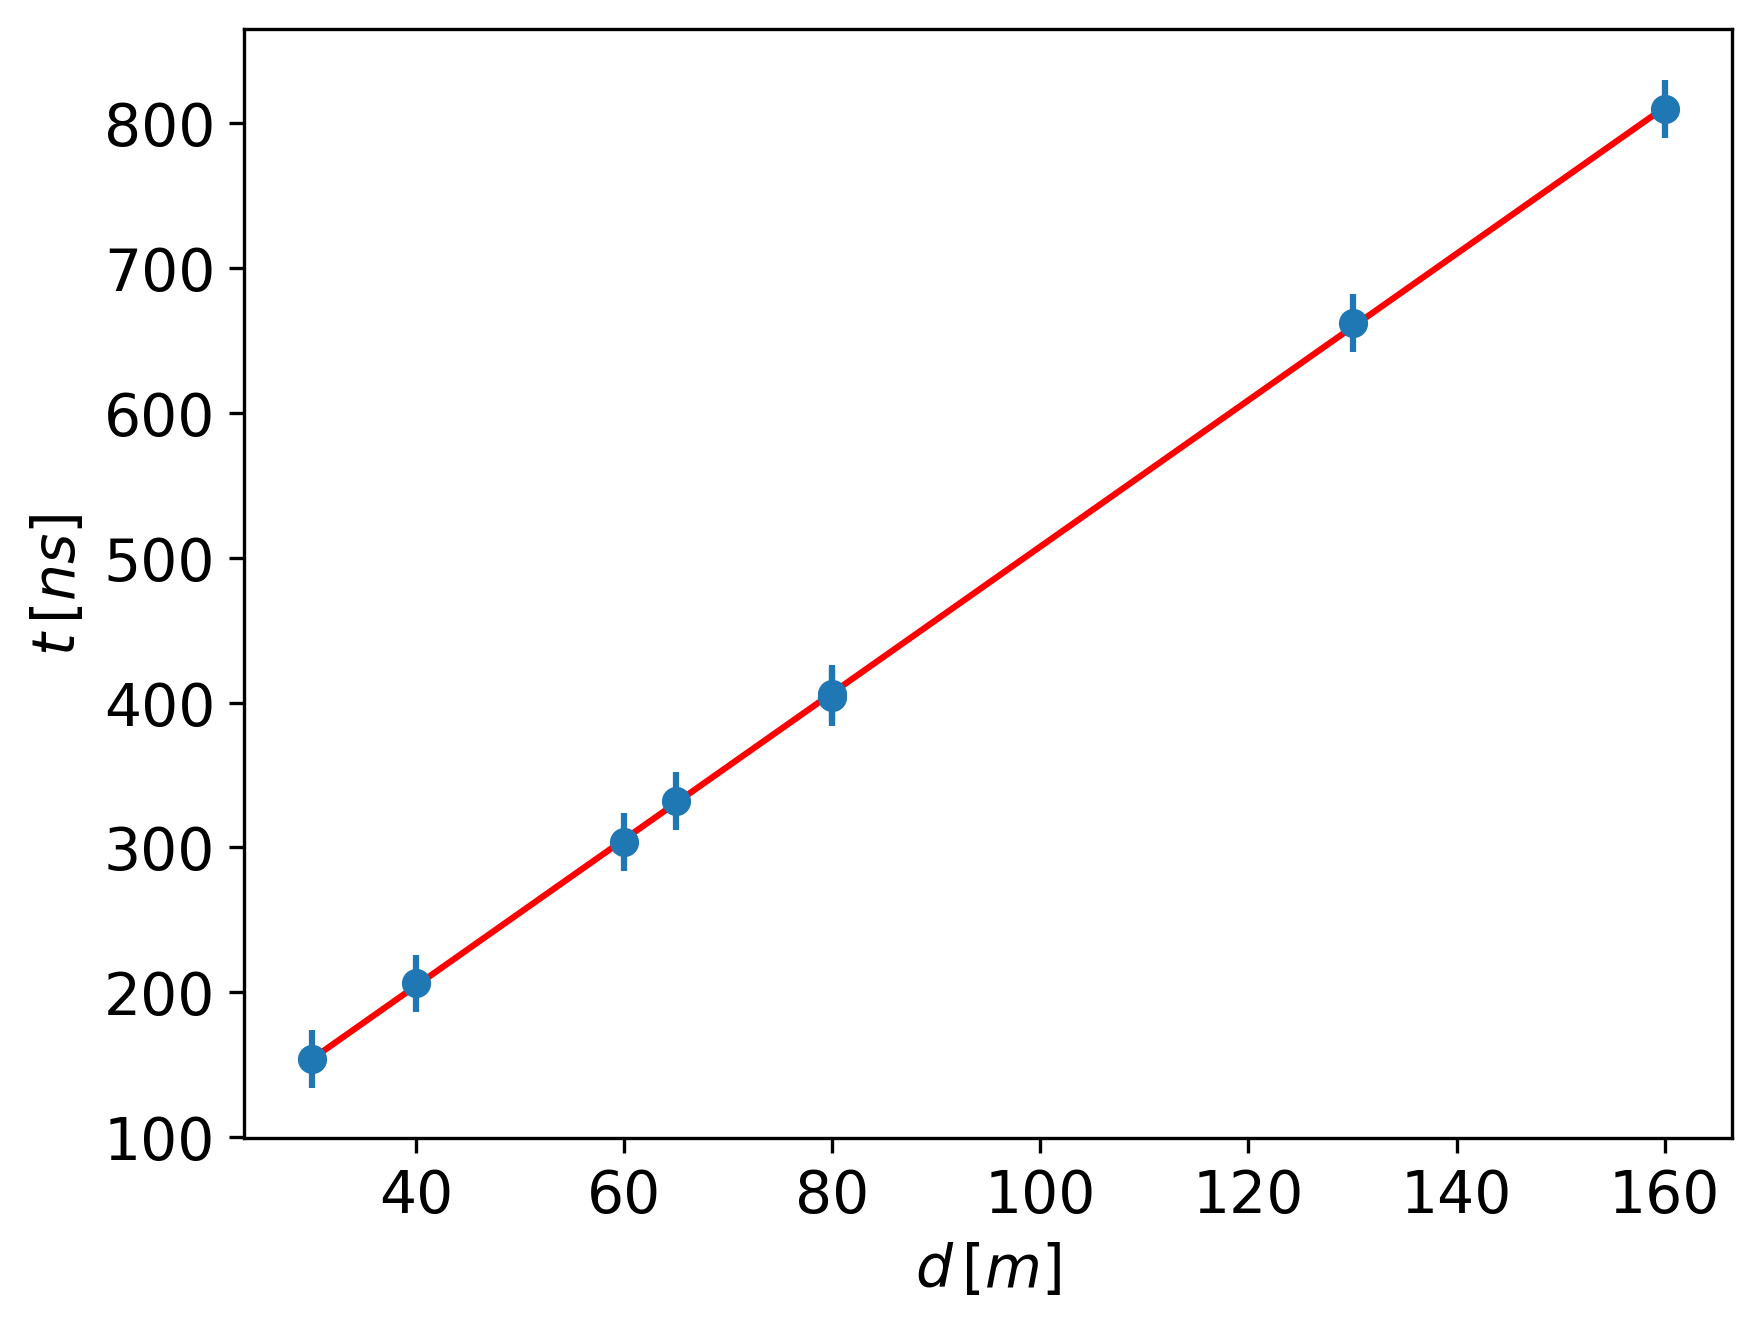
\includegraphics[width=\linewidth]{good_cable_distance}
    \caption{Dobry kabel}
    \label{fig:good_distance}
  \end{subfigure}\hfill
  \begin{subfigure}{0.45\textwidth}
    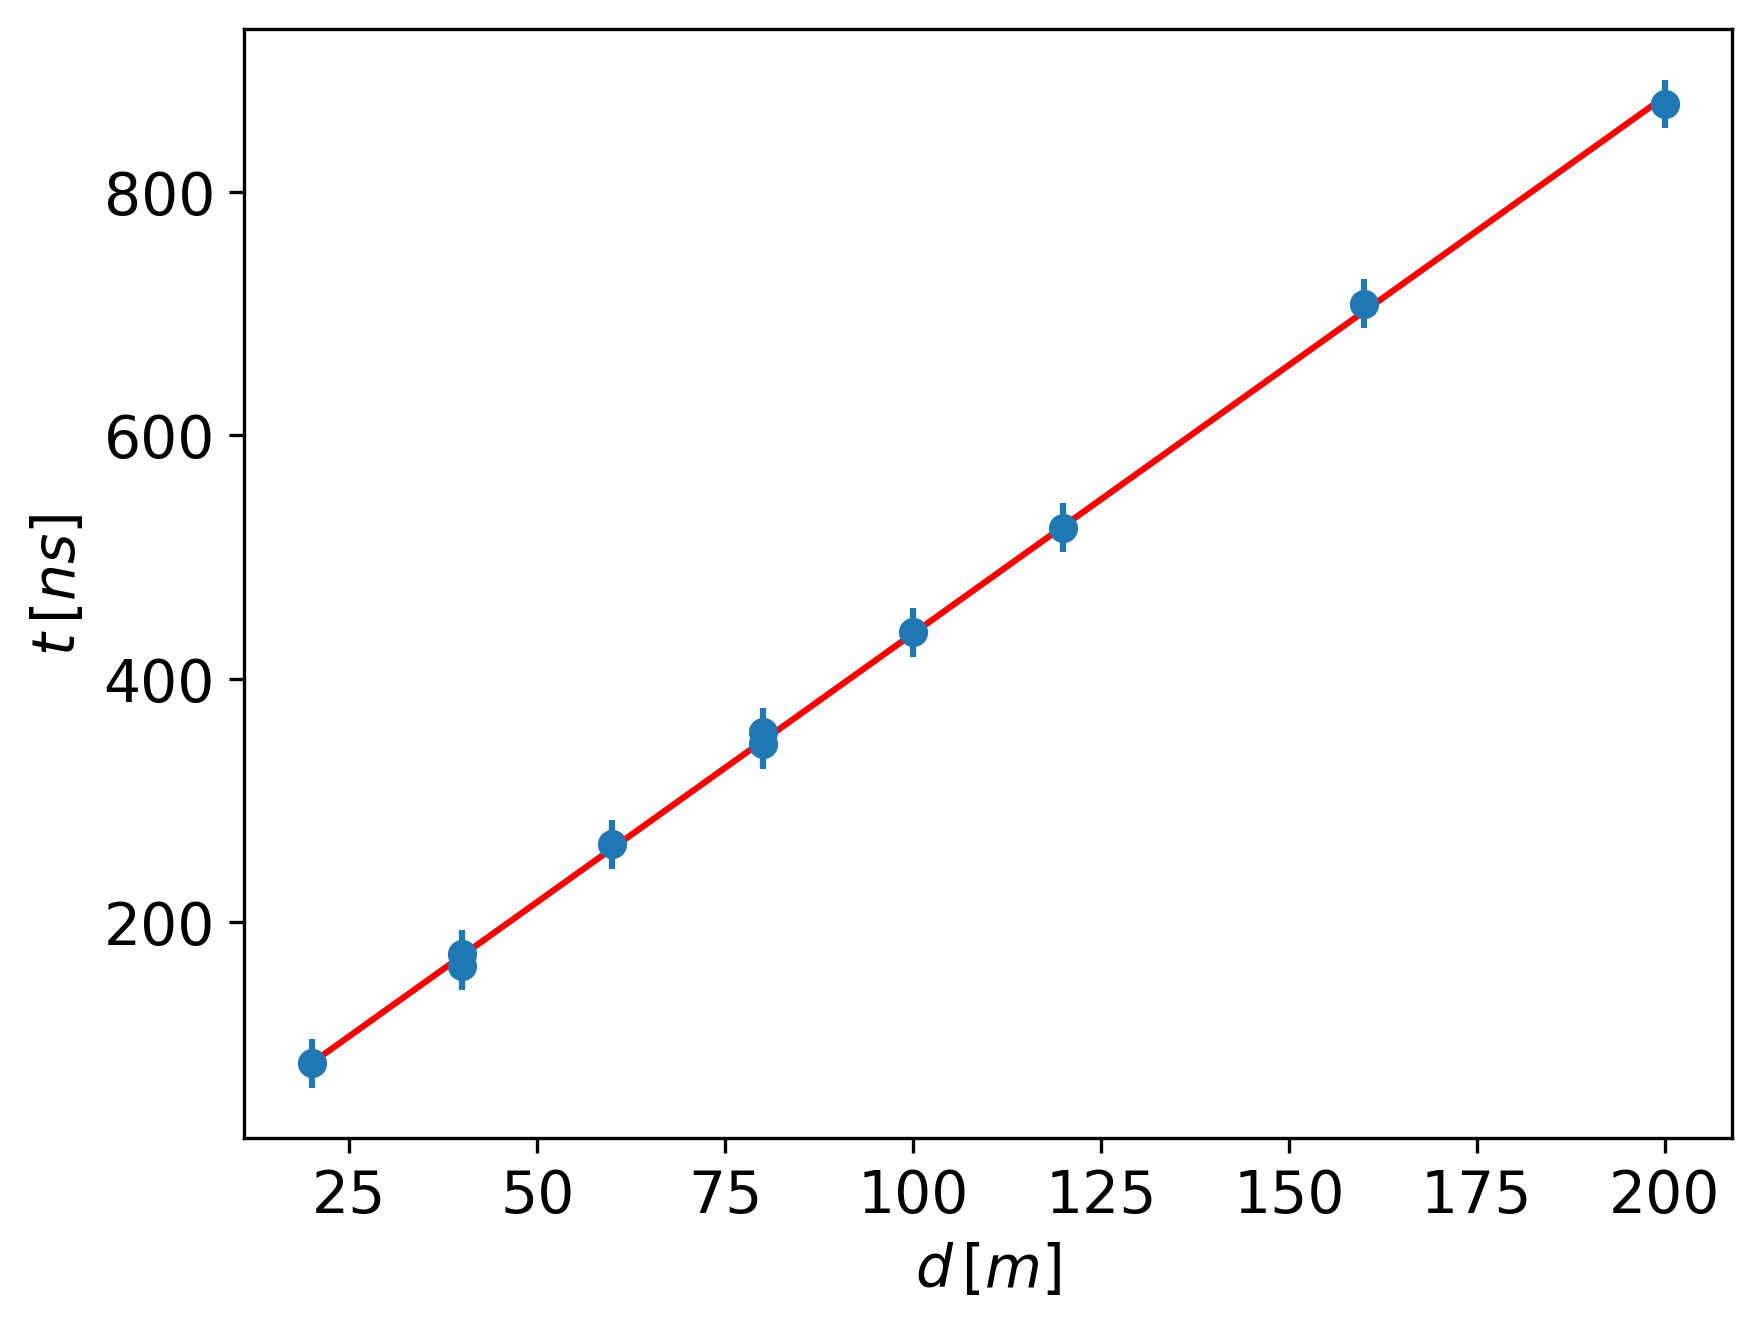
\includegraphics[width=\linewidth]{bad_cable_distance}
    \caption{Zły kabel}
    \label{fig:bad_distance}
  \end{subfigure}
  \caption{Zależność czasu propagacji $t$ od długości kabla $d$. Przedstawiony błąd został przeskalowany 5x dla lepszej widoczności.}
  \label{fig:distance}
\end{figure}

Na podstawie danych z tab.~\ref{tab:good_vs_bad_cable} dopasowaliśmy model liniowy, uzyskując współczynniki

przybliżające nasze pomiary. 
\[
  t = \frac{d}{v} + b,
\]
otrzymujemy prędkości propagacji
\[
  v_{\mathrm{good}}=(9{,}892\pm0{,}032)\times10^{7}\,\mathrm{m\,s^{-1}},\quad
  v_{\mathrm{bad}}=(11{,}341\pm0{,}080)\times10^{7}\,\mathrm{m\,s^{-1}}.
\]

Następnie zmierzyliśmy napięcie odbitego sygnału w~funkcji rezystancji podłączonej do końca kabla.
Błąd pomiarowy oporu wyznaczamy z instrukcji multimetru\cite{resistance} i przedstawiamy go w tabeli z wynikami, podczas gdy błąd napięcia uznajemy za jedną podziałkę oscyloskopu $\Delta U = 0{,}04$.

\begin{table}[H]
  \centering
    \begin{tabular}{c|ccc|ccc}
        \toprule
        \textbf{Nr} &
        \multicolumn{3}{c|}{\textbf{Dobry kabel}} &
        \multicolumn{3}{c}{\textbf{Zły kabel}} \\
        & $R$ [$\Omega$] & $\Delta R$ [$\Omega$] & $U$ [V] & $R$ [$\Omega$] & $\Delta R$ [$\Omega$] & $U$ [V] \\
        \midrule
        1  & 21{,}242  & 0{,}017 & -1{,}20 & 5{,}949   & 0{,}012 & -1{,}76 \\
        2  & 67{,}88  & 0{,}03 & -0{,}08 & 21{,}741  & 0{,}017 & -1{,}16 \\
        3  & 51{,}489  & 0{,}026 & -0{,}40 & 50{,}467  & 0{,}026 & -0{,}44 \\
        4  & 98{,}71  & 0{,}04 &  0{,}32 & 73{,}71  & 0{,}04 & -0{,}04 \\
        5  & 154{,}45 & 0{,}06 &  0{,}80 & 99{,}18  & 0{,}04 &  0{,}28 \\
        6  & 229{,}72 & 0{,}11 &  1{,}08 & 154{,}91 & 0{,}06 &  0{,}68 \\
        7  & 346{,}97 & 0{,}13 &  1{,}40 & 228{,}87 & 0{,}11 &  0{,}96 \\
        8  & 426{,}38 & 0{,}15 &  1{,}60 & 324{,}13 & 0{,}13 &  1{,}20 \\
        9  & 502{,}59 & 0{,}16 &  1{,}68 & 423{,}34 & 0{,}15 &  1{,}48 \\
        10 & 5{,}985   & 0{,}012 & -1{,}92 & 502{,}51 & 0{,}16 &  1{,}52 \\
        \bottomrule
    \end{tabular}
  \caption{Rezystancja $R$ i~napięcie odbitego sygnału $U$ dla dobrego i~złego kabla.}
  \label{tab:good_vs_bad_cable_voltage}
\end{table}

\begin{figure}[H]
  \centering
  \begin{subfigure}{0.45\textwidth}
    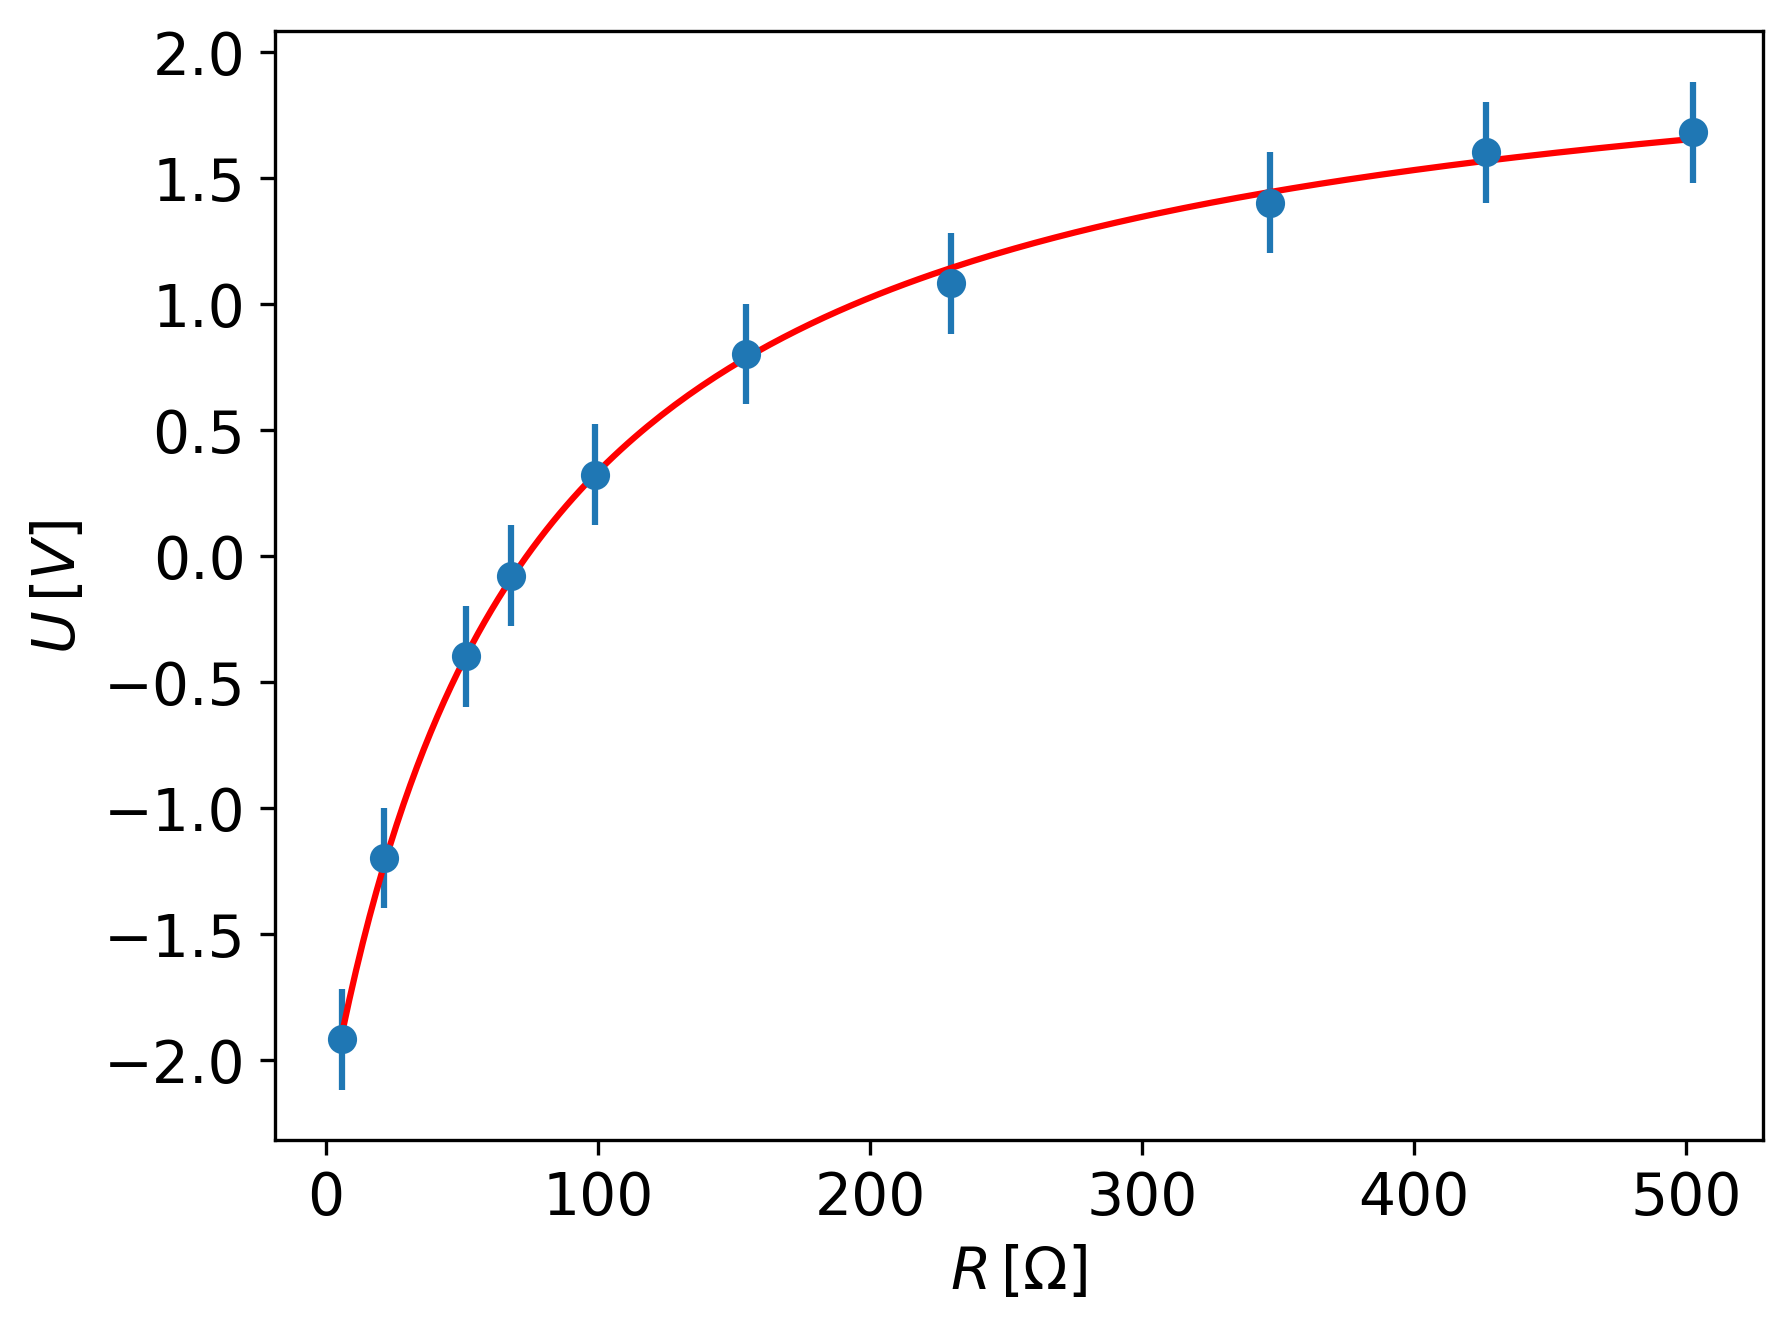
\includegraphics[width=\linewidth]{good_cable_voltage}
    \caption{Dobry kabel}
    \label{fig:good_voltage}
  \end{subfigure}\hfill
  \begin{subfigure}{0.45\textwidth}
    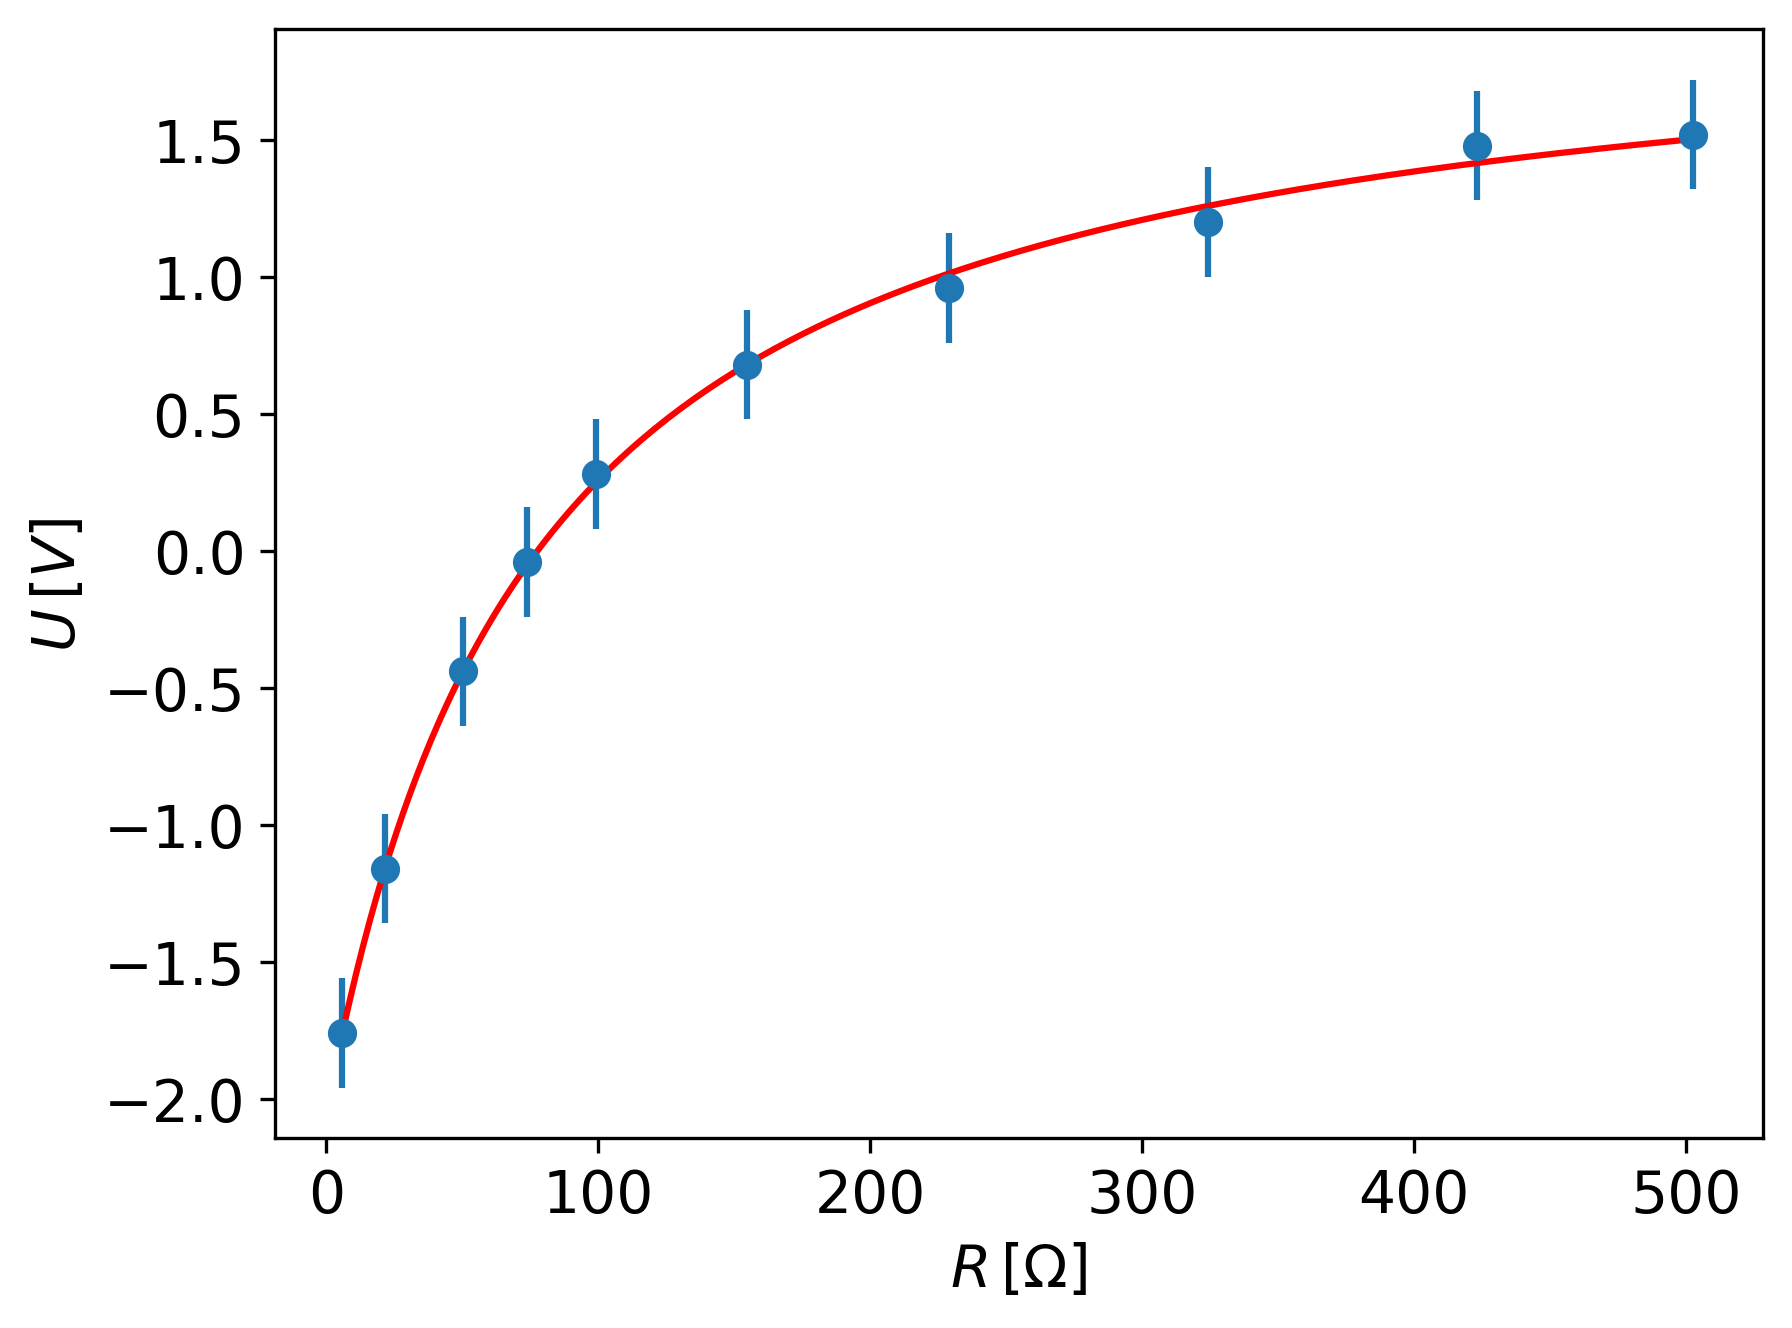
\includegraphics[width=\linewidth]{bad_cable_voltage}
    \caption{Zły kabel}
    \label{fig:bad_voltage}
  \end{subfigure}
  \caption{Zależność napięcia odbitego $U$ od rezystancji obciążenia $R$. Przedstawiony błąd został przeskalowany 5x dla lepszej widoczności.}
  \label{fig:voltage_vs_resistance}
\end{figure}

Otrzymane dane opiszemy zależnością \cite{skrypt}
\[
  U = U_0\,\frac{R_L - Z}{R_L + Z},
\]
\noindent gdzie $U$~-- napięcie odbite, $U_0$~-- napięcie generowane, $R_L$~-- rezystancja obciążenia, $Z$~-- impedancja kabla. 

Do powyższego równania dopasowaliśmy krzywą metodą najmniejszych kwadratów, aby model jak najlepiej opisał zmierzone wartości (tab.~\ref{tab:good_vs_bad_cable_voltage}). W rezultacie otrzymaliśmy parametry
\[
  Z_{\mathrm{good}}=(73{,}9\pm1{,}1)\,\Omega,\quad
  Z_{\mathrm{bad}}=(77{,}7\pm1{,}3)\,\Omega.
\]

Korzystając z~wzorów \cite{skrypt}
\[
  c=\frac{1}{v Z},\qquad l=\frac{Z}{v},
\]
wyznaczamy parametry na jednostkę długości
\begin{align*}
  c_{\mathrm{good}} &= (1{,}367\pm0{,}020)\times10^{-10}\,\mathrm{F\,m^{-1}}, &
  l_{\mathrm{good}} &= (7{,}47\pm0{,}11)\times10^{-7}\,\mathrm{H\,m^{-1}},\\
  c_{\mathrm{bad}}  &= (1{,}135\pm0{,}021)\times10^{-10}\,\mathrm{F\,m^{-1}}, &
  l_{\mathrm{bad}}  &= (6{,}85\pm0{,}12)\times10^{-7}\,\mathrm{H\,m^{-1}}.
\end{align*}

\section{Analiza wyników}
Podczas pomiarów zaobserwowaliśmy, że zły kabel tłumił sygnały silniej niż kabel dobry. Ponadto wyniki dla sprawnego kabla charakteryzowały się mniejszymi niepewnościami, dzięki czemu wyznaczona dla niego impedancja mieści się w~wartości referencyjnej \(75\,\Omega\), podczas gdy dla kabla złego jest ona nieznacznie większa, lecz wciąż miesci się w \(3 \sigma\).

Głównymi źródłami niepewności były rozdzielczości oscyloskopu i~generatora sygnałów. W~pomiarach prędkości propagacji prowadzi to do błędu poniżej \(1\%\). W~detekcji napięcia niepewność jest większa ze względu na trudność jednoznacznego odczytu wartości szczytowej, która w~czasie trwania odbicia nieznacznie maleje. Dodatkowo niewielki błąd pochodzi z~rozdzielczości multimetru użytego do pomiaru rezystancji obciążenia. Wpływ dodatkowych połączeń kablowych uznaliśmy za pomijalny.

\vspace{1 in}

\begin{thebibliography}{2}

\bibitem{resistance}
Instrukcja multimetru RIGOL DM3058E \url{http://pracownie1.fuw.edu.pl/przyrzady/Multimetr_Rigol_DM3058_UserGuide_EN.pdf}
\bibitem{skrypt}
Piotr Fita, \emph{Kabel koncentryczny}, skrypt laboratoryjny, Uniwersytet Warszawski.

\end{thebibliography}

\end{document}
